\section{A Machine Model for Line-rate Switches}
\label{s:absmachine}

\begin{figure*}[!t]
  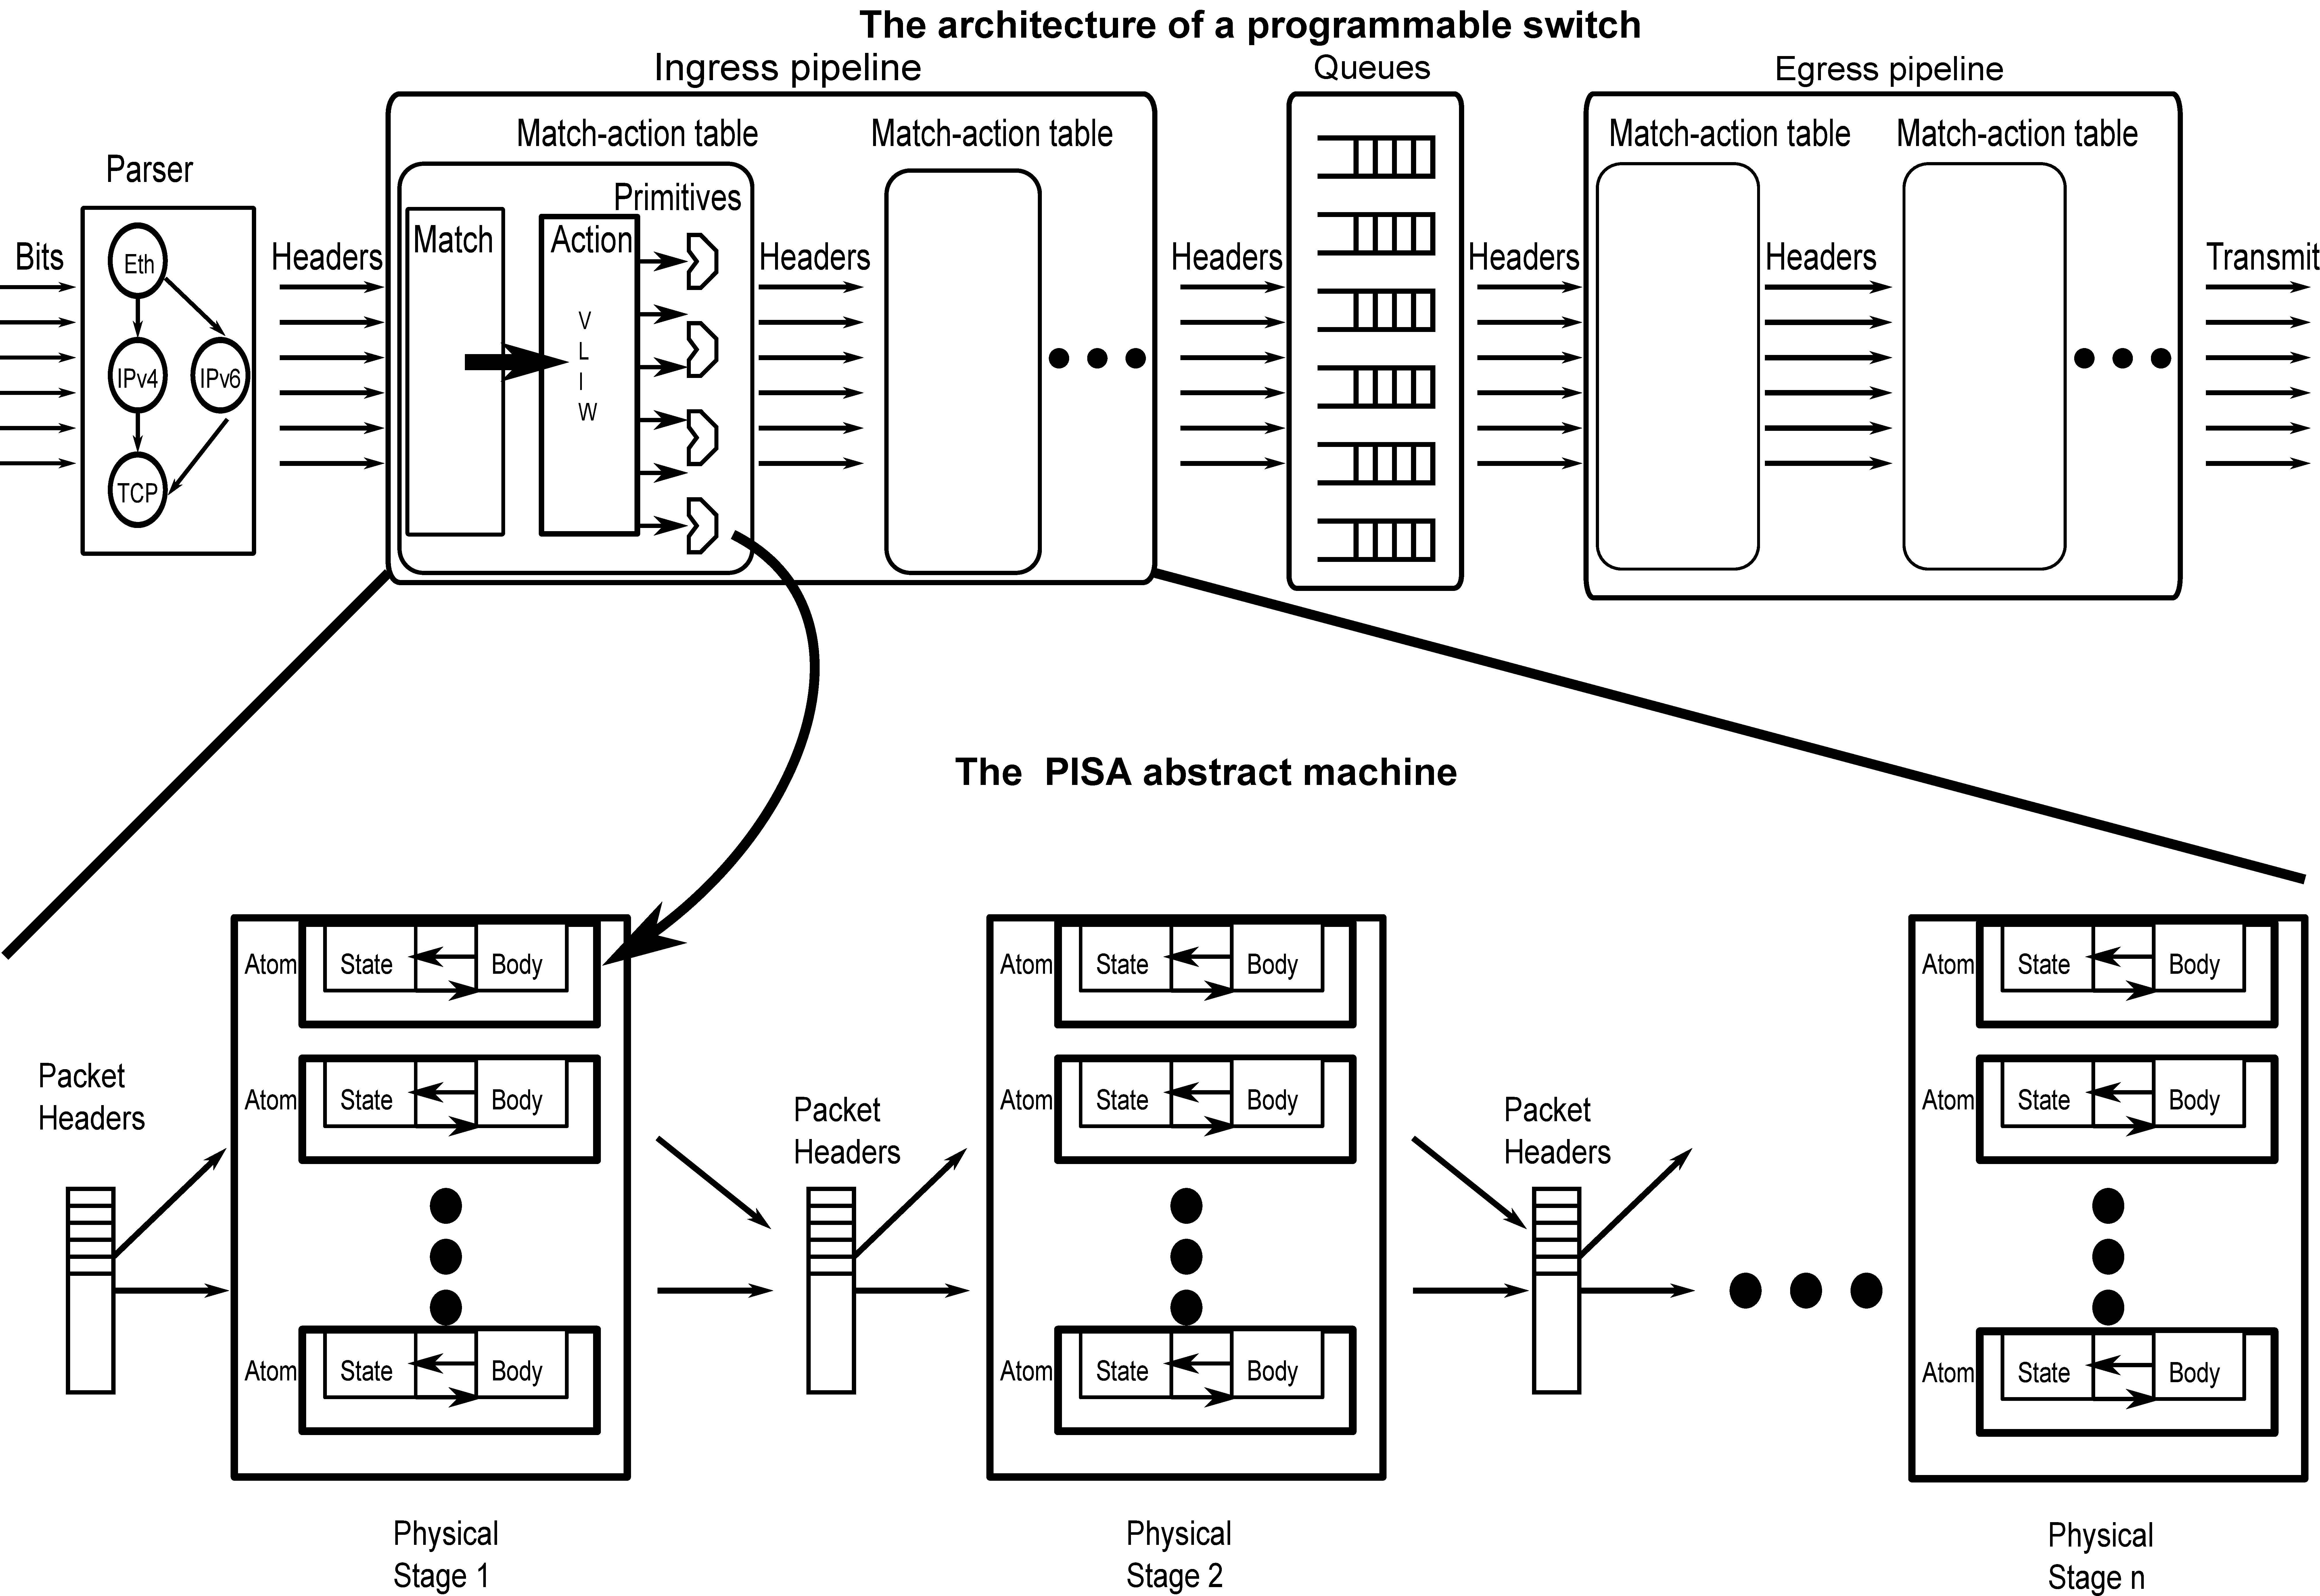
\includegraphics[width=\textwidth]{pisa.pdf}
  \caption{The \absmachine abstract machine and its relationship to
  programmable switch architectures.}
  \label{fig:switch}
\end{figure*}

%TODO: Don't call this an abstract machine. I think that's part of the problem.
% Altenate name: architecture, machine model, and ...?
% People think of this as an IR / portable abstract machine, as opposed to an actual model of the hardware.
% I think that's what triggers the comparisons to NetASM.
% MA: I agree. 

% This section describes \absmachine (Protocol-Independent Switch
% Architecture), a family of abstract machines for programmable
% switches.  \footnote{The term PISA was briefly introduced in a
%   workshop talk~\cite{nick_p4}.  Here, we develop PISA into a
%   \textit{fully executable} computational model for programmable
%   switches.} \absmachine abstracts and generalizes line-rate
% programmable switch architectures, such as RMT~\cite{rmt}, Intel's
% FlexPipe~\cite{flexpipe}, and Cavium's XPliant Packet
% Architecture~\cite{xpliant} and \absmachine machines serve as compiler
% targets for \pktlanguage programs.

This section describes \absmachine (Protocol-Independent Switch
Architecture), a machine model for programmable line-rate switches
that serves as the compiler target for \pktlanguage
programs.\footnote{The term PISA was introduced in a workshop
  talk~\cite{nick_p4}.  Here, we develop PISA into a \textit{fully
    executable} machine model for programmable switches.\MA{This
    sounds weird. Lets either get rid of this footnote, or just call
    it Banzxai.}}  \absmachine is inspired by recent programmable
switch architectures such as RMT~\cite{rmt}, Intel's
FlexPipe~\cite{flexpipe}, and Cavium's XPliant Packet
Architecture~\cite{xpliant}. \absmachine abstracts these architectures
and extends them with stateful processing units which are used to
implement data-plane algorithms. These processing units, called {\em
  atoms}, precisely model the set of operations that a hardware target
can execute at line-rate, and act as the low-level instruction set for
the \pktlanguage compiler.

% \absmachine machines serve as compiler targets for \pktlanguage
% programs.


% We chose this approach relative to targeting actual hardware for two reasons.
% First, programmable switches are rapidly evolving, so targeting one in
% particular risks obsolescence. Second, the software ecosystem to program these
% chips is heavily in flux. We do, however, address the practicality of these
% \absmachine machines by quantifying their chip area overhead
% in\S\ref{ss:atoms}.

% MA: Lets get rid of the above paragraph; we can explain these points
% in the intro and evaluation.

\subsection{Programmable switch architectures}
Packets arriving to a programmable switch~(Figure~\ref{fig:switch})
are parsed by a programmable parser that turns packets into header
fields. These header fields are first processed by an ingress pipeline
consisting of match-action tables arranged in stages. Processing a
packet at a stage may modify its header fields as well as some
persistent state at that stage. Each stage only has access to its
local state. To share state between stages, it must be carried in
packet headers.

Following the ingress pipeline, the packet is queued. Once the packet
is dequeued by the switch scheduler, it is processed by a similar
egress pipeline before being transmitted.

To reduce chip area, the ingress and egress pipelines are shared
across switch ports.  Each pipeline needs to handle aggregate traffic
belonging to all ports on the switch, at all packet sizes.  For
instance, a 64-port switch with port speeds of 10 Gigabits/second and
a minimum packet size of 64 bytes needs to process around a billion
packets per second~\cite{rmt}.  Equivalently, with a clock frequency
of 1 GHz, each pipeline stage needs to process one packet every clock
cycle (1 ns).  The need to handle one packet per clock cycle is
typical because switches are designed for the highest port density and
speed supported by the switching chip. We assume one packet per clock
cycle throughout the paper.\footnote{For concreteness, we assume a 1
  GHz clock frequency.}

Having to process a packet every clock cycle in each stage greatly
curtails the operations that can be performed on each packet. In
particular, any packet operation that modifies state that is visible
to the next packet must execute fully in a single clock cycle (see
$\S$\ref{s:atoms} for details). Because of this restriction, in
contrast to software routers, programmable switching chips provide a
small set of processing units or primitives for manipulating packets
and state in a stage. These processing units determine what algorithms
can run on the switch at line-rate. 

The technical challenge here is to determine primitives that enable a
broad range of data-plane algorithms to be implemented, and build a
compiler for mapping a user-friendly description of an algorithm to
these low-level primitives.


%The technical challenge here is to build a compiler that can determine
%the primitives needed to implement a data-plane algorithm from a
%user-friendly description of the algorithm.

\subsection{The \absmachine abstract machine}

\absmachine (the bottom half of Figure~\ref{fig:switch}) models a
switch pipeline such as the ingress or egress pipeline. A pipeline in
\absmachine consists of a number of stages executing synchronously on
every time step. An incoming packet is processed by each stage and
handed off to the next, until it exits the pipeline. Each stage has
one time step of latency, which in our case is 1 ns.\MA{This isn't
  necessary for the hardware, right? A stage can take more than one
  clock cycle. Do we need to say the latency is 1 ns?} \absmachine
only models components pertinent to data-plane algorithms.  It models
the computation within a match-action table in a stage (i.e., the
action half of the match-action table), but not the match semantics
(e.g., direct, or ternary). One could embed these actions in a
standard match-action pipeline by making them default
actions~\cite{p4spec} for each table.  \MA{I don't quite understand
  this. Say the computation involves looking up some state (e.g., the
  last virtual finish\_time in fair queuing). Wouldn't the lookup be
  part of the transaction?}  \absmachine does not model packet parsing
and assumes that packets arriving to it are already parsed.

\subsection{Atoms: \absmachine's processing units}
\label{ss:atoms}

In \absmachine, each pipeline stage contains a vector of
\textit{atoms}. All atoms in this vector execute in parallel on every
time step.  Informally, an atom is an atomic unit of packet processing
supported natively by a \absmachine machine. Atoms can optionally
modify persistent state stored on the switch and constitute the
machine's instruction set.  In contrast to instruction sets for CPUs,
GPUs, DSPs, and NPUs, the atoms for a \absmachine machine need to be
substantially richer to enable useful operations at line-rate. We
explain this through an example below.

Let us assume we need to atomically increment a state variable stored
on the switch to count packets. Naively, this can be done with
hardware support for three simple operations: \textit{reading} some
memory from one pipeline stage, \textit{adding} one in the next, and
\textit{writing} it to memory in the third. However, this doesn't
provide atomicity. To see why, assume packet 1 increments the counter
from 0 to 1 by transiting the read, add, and write stages at times 1,
2, and 3 respectively.  If packet 2 arrives at the read stage at time
2, it will increment the counter again from 0 to 1, when it should be
2. \MA{I think we need to make a distinction between a stage and a
  clock cycle. Your example does not need three pipeline stages. The
  point is that the three operations must occur atomically in the same
  clock cycle, because the result of the operation is needed for
  packet 2.}  Locks are a potential solution. However, locking causes
packet 2 to wait during packet 1's increment, and the switch no longer
sustains line rate, which it is expected to regardless of the input
workload.\footnote{Wait-free objects~\cite{herlihy_wait} are an
  alternative to locking, but are typically too complicated for
  hardware.}

In this architecture, the only way to provide an atomic increment is
to expressly support it in hardware by reading memory, incrementing it
and writing it back in a single stage within one clock cycle. The same
observation applies to any line-rate atomic operation---not just an
increment.  This motivate our representation of atoms as a body of
sequential code. An atom completes execution of the entire body of
code and modifies a packet before processing the next packet.  An atom
may also contain internal state that is local to that atom alone and
persists across packets.  

Using this representation, a switch counter that wraps around at 100
can be written as the atom below.\footnote{We use {\tt p.x} to
  represent field {\tt x} within a packet {\tt p} and {\tt x} to
  represent a state variable {\tt x} that persists across packets.}
\begin{lstlisting}[style=customc, numbers=none, frame=none]
if (counter < 99)
  counter++;
else
  counter = 0;
\end{lstlisting}
Similarly, a stateless operation like setting a packet field (e.g. P4's {\tt
modify\_field} primitive~\cite{p4spec}) can be written as the atom:
\begin{lstlisting}[style=customc, numbers=none, frame=none]
  p.field = value;
\end{lstlisting}
Table~\ref{tab:templates} provides more examples of atoms.

We note that---unlike stateful atomic operations such as increment
that modify persistent state--- stateless operations can be supported
by providing a set of basic stateless operations such as packet field
arithmetic. Consider, for instance, the operation pkt.f1 = pkt.f2 +
pkt.f3 - pkt.f4. Because this operation doesn't modify state that is
visible to the next packet, it can be implemented by adding in one
stage, and the subtracting in the next, unlike the increment.

%%\absmachine generalizes several aspects of existing programmable switch
%%architectures. The vector of atoms in each stage generalizes RMT's very-large
%%instruction-word (VLIW)~\cite{rmt} that executes primitive actions on packet
%%fields in parallel. Internal state within an atom models persistent switch
%%state such as meters, counters, and P4's register abstraction~\cite{p4spec} in
%%a unified manner. We assume all state is initialized by the switch control
%%plane, which we don't explicitly model in \absmachine.
%%
\subsection{Computational limits}
\label{s:atomConstraints}

%%Atoms in \absmachine execute on every time step, reading all packet fields at
%%the beginning and writing all packet fields at the end of a time step. To
%%prevent data races, \absmachine forbids two atoms in a stage from writing to
%%the same packet field.
%%We impose two such constraints that
%%distinguish \absmachine from software routers~\cite{click} and network
%processors~\cite{ixp4xx} that sacrifice determinism for programmability.

To provide line-rate performance, atom bodies must be suitably
constrained.  When implemented in digital logic, the atom body must
finish execution within one clock cycle (1 ns for a 1 GHz clock
frequency). We constrain atom bodies by defining {\it atom templates}
(\S\ref{ss:code_gen}).  An atom template is a program that always
terminates and specifies exactly how the atom is executed. One example
is an ALU with a restricted set of primitive operations to choose from
(Figure~\ref{fig:alu_diag}). Atom templates allow us to create
\absmachine machines with different atoms.  In practice, atom
templates will be designed by an ASIC engineer and exposed as a
machine's instruction set~(\S\ref{ss:targets}).  As programmable
switches evolve, atoms will evolve as well.  However, atoms cannot be
arbitrarily complex: the line rate is inversely proportional to an
atom's execution latency~(\S\ref{ss:perfprog}).

\subsection{Resource limits}
\label{s:resource}

For any real architecture, we also need to limit the number of atoms
in each stage (the pipeline width) and the number of stages in the
pipeline (the pipeline depth). This is similar to the limits on the
number of stages, number of tables per stage, and amount of memory per
stage in programmable switch architectures such as RMT and
FlexPipe~\cite{lavanya_compiler}.
